\input{../YKY-preamble.tex}
\setmainfont[BoldFont=AlibabaSans-Regular.otf,ItalicFont=AlibabaSans-LightItalic.otf]{AlibabaSans-Light.otf}
	
\usepackage[active,tightpage]{preview}		% for continuous page(s)
\renewcommand{\PreviewBorder}{0.5cm}
\renewcommand{\thempfootnote}{\arabic{mpfootnote}}

\usepackage[absolute,overlay]{textpos}		% for page number on upper left corner

\usepackage{color}
\usepackage{mathtools}
\usepackage[hyperfootnotes=false]{hyperref}

% \usepackage[backend=biber,style=numeric]{biblatex}
% \bibliography{../AGI-book}
% \renewcommand*{\bibfont}{\footnotesize}

\usetikzlibrary{shapes}
\usepackage[export]{adjustbox}				% ??
\usepackage{bm}
\usepackage{verbatim} % for comments
% \usepackage{newtxtext,newtxmath}	% Times New Roman font

% \numberwithin{equation}{subsection}

\newcommand{\underdash}[1]{%
	\tikz[baseline=(toUnderline.base)]{
		\node[inner sep=1pt,outer sep=10pt] (toUnderline) {#1};
		\draw[dashed] ([yshift=-0pt]toUnderline.south west) -- ([yshift=-0pt]toUnderline.south east);
	}%
}%

% Tic-Tac-Toe symbols
% \newcommand{\bO}[0]{\raisebox{-0.2em}{\textbf{O}}}
% \newcommand{\Xb}[0]{\raisebox{-0.2em}{\textbf{X}}}

%\DeclareSymbolFont{symbolsC}{U}{txsyc}{m}{n}
%\DeclareMathSymbol{\strictif}{\mathrel}{symbolsC}{74}
\DeclareSymbolFont{AMSb}{U}{msb}{m}{n}
\DeclareSymbolFontAlphabet{\mathbb}{AMSb}
% \setmathfont{Latin Modern Math}

% \newcommand{\highlight}[1]{\colorbox{pink}{$\displaystyle #1$}}

% \newcommand{\emp}[1]{{\color{violet}\textbf{#1}}}
\let\oldtextbf\textbf
\renewcommand{\textbf}[1]{\textcolor{blue}{\oldtextbf{#1}}}

\newcommand*\cryLaughFace{$\vcenter{\hbox{\includegraphics[scale=0.08]{../crying-laughing.jpg}}}$}
\newcommand{\underconst}{\includegraphics[scale=0.5]{../2020/UnderConst.png}}
\newcommand{\KBsymbol}{\vcenter{\hbox{\includegraphics[scale=1]{../KB-symbol.png}}}}
\newcommand{\witness}{\scalebox{0.6}{$\blacksquare$}}
% \newcommand{\Heytingarrow}{\mathrel{-}\mathrel{\triangleright}}
% \providecommand\Heytingarrow{\relbar\joinrel\mathrel{\vcenter{\hbox{\scalebox{0.75}{$\rhd$}}}}}

\begin{document}

\begin{preview}

\cc{
\title{\vspace{-1.5cm} \bfseries\color{blue}{\Large 强化学习的「思维空间延拓」}}
}{
\title{\vspace{-1.5cm} \bfseries\color{blue}{\Large ``Mental-Space Continuation'' \\
		of Reinforcement Learning}}
}

% \author{YKY} % Your name
\date{\vspace{-2cm}} % Date, can be changed to a custom date

\maketitle

\setcounter{section}{-1}

% (1) Circled page number on upper left corner
\begin{textblock*}{5cm}(2.1cm,2.3cm) % {block width} (coords) 
{\color{red}{\large \textcircled{\small 1}}}
\end{textblock*}

\begin{minipage}{\textwidth}
\setlength{\parskip}{0.4\baselineskip}

\cc{
	在传统的强化学习里,「环境」只包含 physically observable 的外在环境。\\
	我提出将 RL 延续到\textbf{内在的}思维空间。
}{
	In conventional RL, the \textbf{environment} is physically observable.  I propose to extend it to the \textbf{internal} mental space.
}

\cc{
	从传统 RL 的角度: 人伸手拿苹果,苹果是\textbf{奖励},伸手是\textbf{动作}。\\
	这些都是可以在环境中\textbf{观察}到的:
}{
	From the traditional RL perspective:  an agent reaches out for an apple, the apple is the \textbf{reward}, moving the arm is an \textbf{action}.  These are all \textbf{observables}:
}
\begin{equation}
\vcenter{\hbox{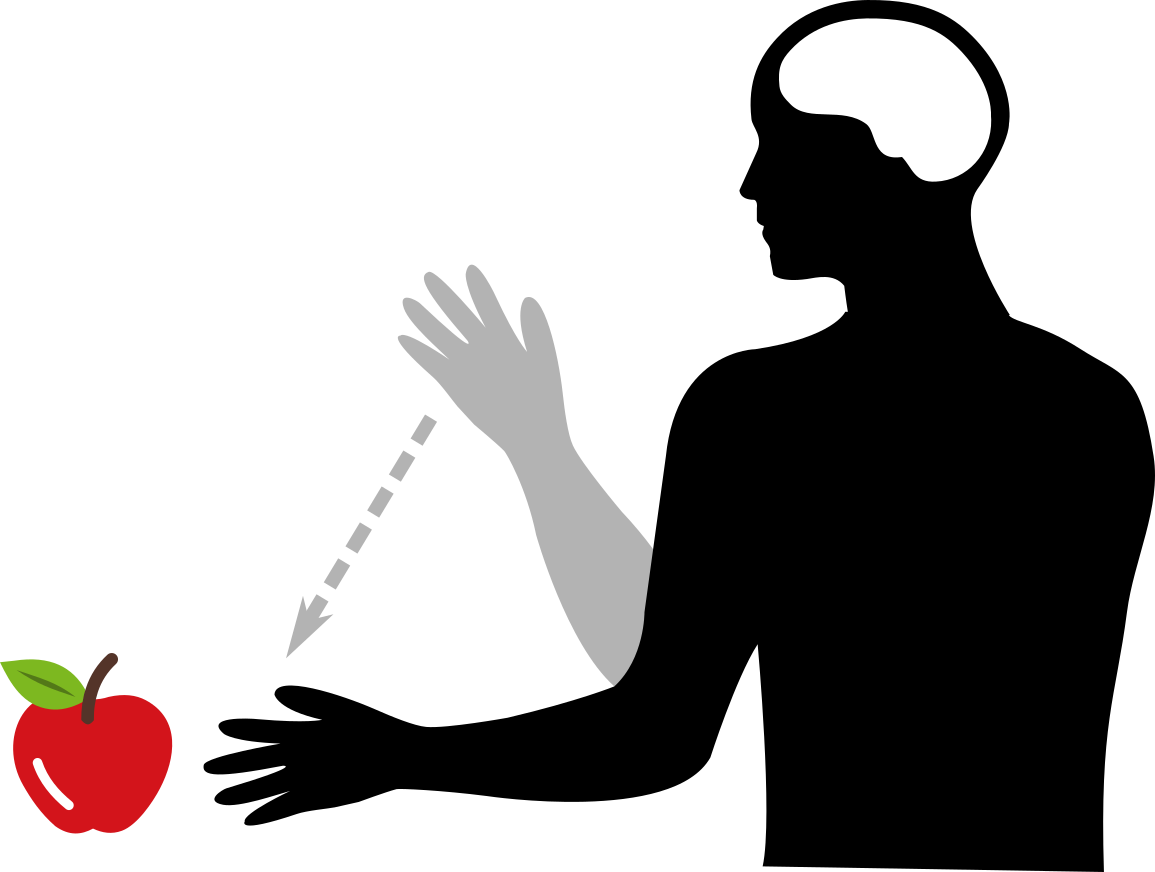
\includegraphics[scale=0.5]{man-grab-apple.png}}}
\end{equation}

\cc{
	强化学习的基础是 \textbf{Bellman equation}, 它可以看成是一条「\textbf{递归}」的方程:
}{
	The foundation of RL is the \textbf{Bellman equation}.  It can be viewed as a \textbf{recursive} formula:
}
\begin{equation}
\boxed{\mbox{\cc{当前状态}{Current state}}} \quad V(x_0) = \max _a \{ R + \gamma V(x_1)\} \quad \boxed{\mbox{\cc{下一状态}{Next state}}}
\end{equation}
\cc{
	它将 \textbf{终点}状态的\textbf{价值}「反向传递\footnote{注意这不同于神经网络的 back-prop.}」到 终点前一步的状态的价值,就像下棋的情况,可以一直追溯到第一步棋的价值:
}{
	It propagates the final state's reward \textbf{back} to the previous state, and the state before that... just like in a chess game... and so on until the very first move:
}
\begin{equation}
\vcenter{\hbox{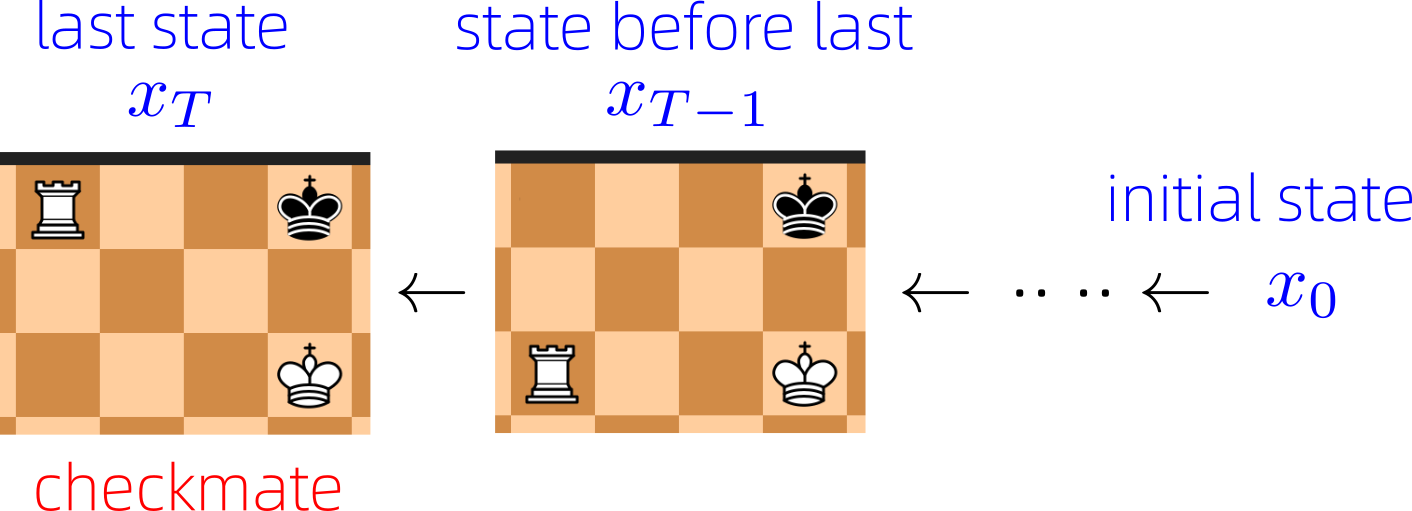
\includegraphics[scale=0.7]{checkmate-sequence.png}}}
\end{equation}

\cc{
	换句话说,获得苹果的价值,反向传递到「伸手取苹果」这动作的价值。 \\
	So far so good. \\
	而同样地,我们可以继续反向传递到决定「伸手取苹果」之前的一连串\textbf{思维}:
}{
	In other words, the reward of getting an apple \textit{back-propagates}\footnote{Note that this is not the same as ``back-prop'' in deep learning.} to the action of reaching out an arm for the apple.  So far so good.  But we can continue this process back to the \textbf{chain of thoughts} that decided to reach for an apple:
}
\begin{equation}
{\color{blue}\mbox{\cc{我肚饿}{hungry}}} \rightarrow {\color{blue}\mbox{\cc{我要找食物}{need to find food}}} \rightarrow {\color{blue}\mbox{\cc{我看见一只苹果}{see an apple}}} \rightarrow {\color{blue}\mbox{\cc{苹果是食物}{apple is food}}} \rightarrow ....
\end{equation}
\cc{
	换句话说,将\textbf{内部}的思维状态「反转」,看成跟\textbf{外部}的状态,是\uline{同等的地位}:
}{
	In other words, we turn our \textbf{internal} mental states ``inside-out'', viewing them \uline{on an equal footing} as \textbf{external} states:
}
\begin{equation}
\vcenter{\hbox{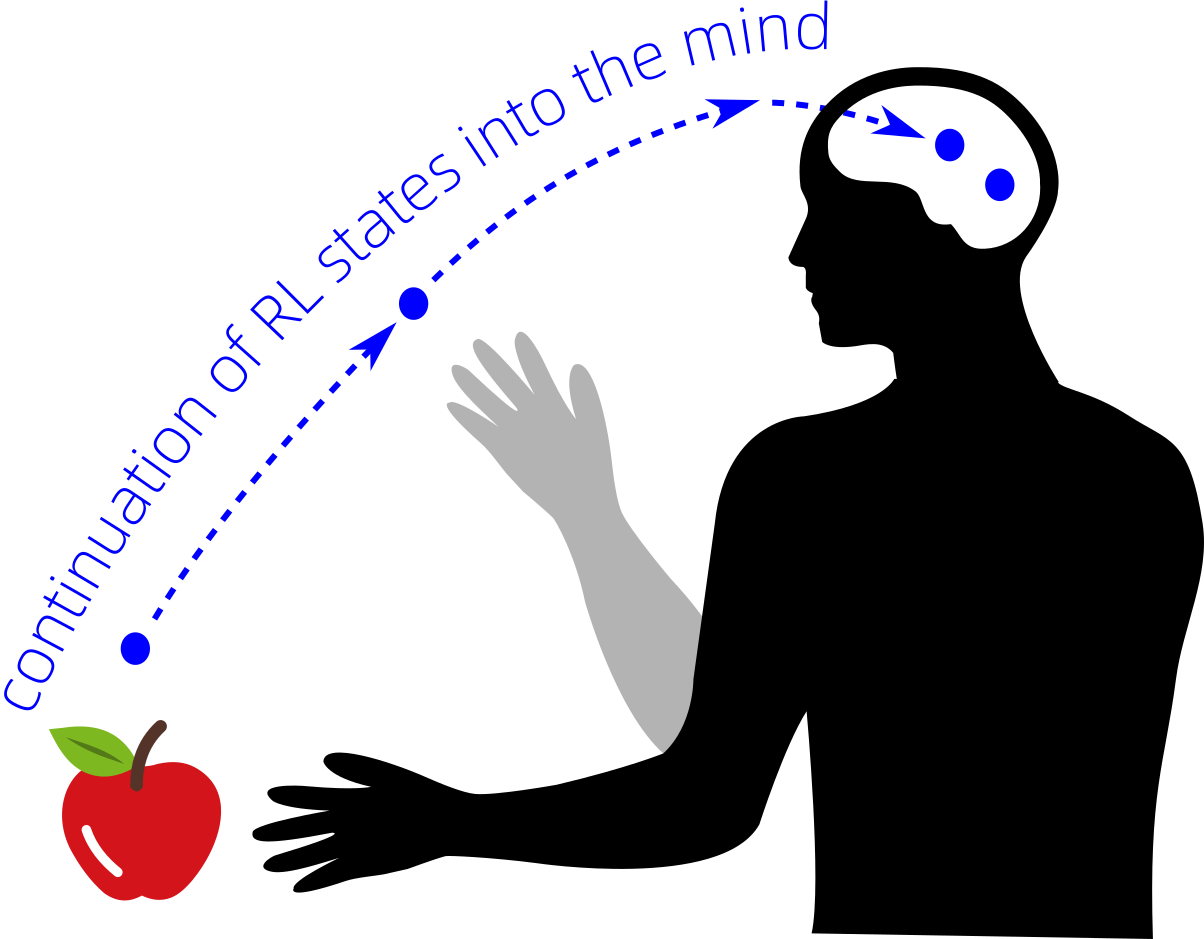
\includegraphics[scale=0.5]{man-grab-apple-2.png}}}
\end{equation}
\cc{
	而这跟象棋的价值函数的反向传递是\uline{完全一样的}。 换句话说,我们可以用强化学习的算法,学习思维空间的内容,提供了 AGI 严谨的基础。
	}{
	And this is \uline{exactly analogous} to the propagation of rewards in a chess game.  In other words, we can apply techniques of RL to learn the contents of mental space, with a very rigorous foundation.
}

\end{minipage}
\end{preview}

\begin{preview}
\begin{minipage}{\textwidth}
\setlength{\parskip}{0.4\baselineskip}

\begin{textblock*}{20cm}(2.1cm,2cm) % {block width} (coords) 
	{\color{red}{\large \textcircled{\small 2}}}
	\hspace{8cm}
	\color{blue}{\footnotesize \cc{强化学习的「思维空间延拓」}{Mental-Space Continuation of RL}}
\end{textblock*}

\vspace*{0.3cm} 

\subsubsection{Learning of logic rules under RL}

\cc{
	将 外部和内部状态 \textbf{统一处理}的做法,在哲学上也没有问题,因为其实 brain states 也是物理状态,只是肉眼看不到而已。 大脑状态 即是 神经元群的激活状态,它们之间的 transitions 是由神经\textbf{权重}决定的,而这些权重又是由 \textbf{Hebbian learning} 学习的(至少根据我们现时最好的理解)。 
}{
	The approach of unifying internal and external states is philosophically entirely sound, as ``brain states'' are physical states too, and their transitions are learned via \textbf{Hebbian learning}.}

\cc{
	而 强化学习 又是怎样\textbf{学习} 逻辑内容? \textbf{动作} 就是由一个逻辑状态 转移到另一个 逻辑状态,也可以看成是 由一些命题 \textbf{推导}出 一个新的命题,那就是 逻辑 \textbf{rule}.  我们要在很多 动作(逻辑 rules)之中选取最好的 动作。 换句话说,要在当前状态下可以执行的 rules 之中选取最好的一个或多个 rule(s).  例如「我很肚饿$\rightarrow$我要找食物」是一条正确的 rule;「我很肚饿$\rightarrow$我要吃屎」就比较差了 \cryLaughFace
}{
	So how does RL learn logical content?  An \textbf{action} here is a transition from one logic state (set of propositions) to another, ie, a logic \textbf{rule}.  The agent tries to learn the best actions (= logic rules) among all possible rules that are \textit{applicable} to the current state.  For example:
}
\begin{equation}
\mbox{I'm hungry} \rightarrow \mbox{need to find food}
\end{equation}
is a good rule;
\begin{equation}
\mbox{hungry} \rightarrow \mbox{eat feces}
\end{equation}
is not so good.

\cc{
	而 强化学习 的好处是: 理论上,它可以在无限的思维空间里 学到非常\textbf{抽象}的 rules,情形就像它在复杂的游戏\textbf{迷宫}里,学到破解的方法。
}{
	The advantage of this RL framework is that it may be able to learn highly \textbf{abstract} rules from the vast mental space, just like it learns to find solutions out of complicated \textbf{mazes} in Atari games.
}

\setcounter{mpfootnote}{1}
\cc{
	在经典 AI 里已有研究过 逻辑 rules 的 combinatorial 搜寻,例如有这种形式的搜寻树:(但注意这并不等同于 \textbf{RL 状态空间}的形状 \footnote{我有空的时候会再思考一下: RL 思维状态空间 长什么样子,它有什么特性? 它跟游戏迷宫 有什么相似/不同?})
}{
	In classical AI, the \textbf{combinatorial} search of logic rules has been studied, with \textbf{search trees} like this:
}
\begin{equation}
\vcenter{\hbox{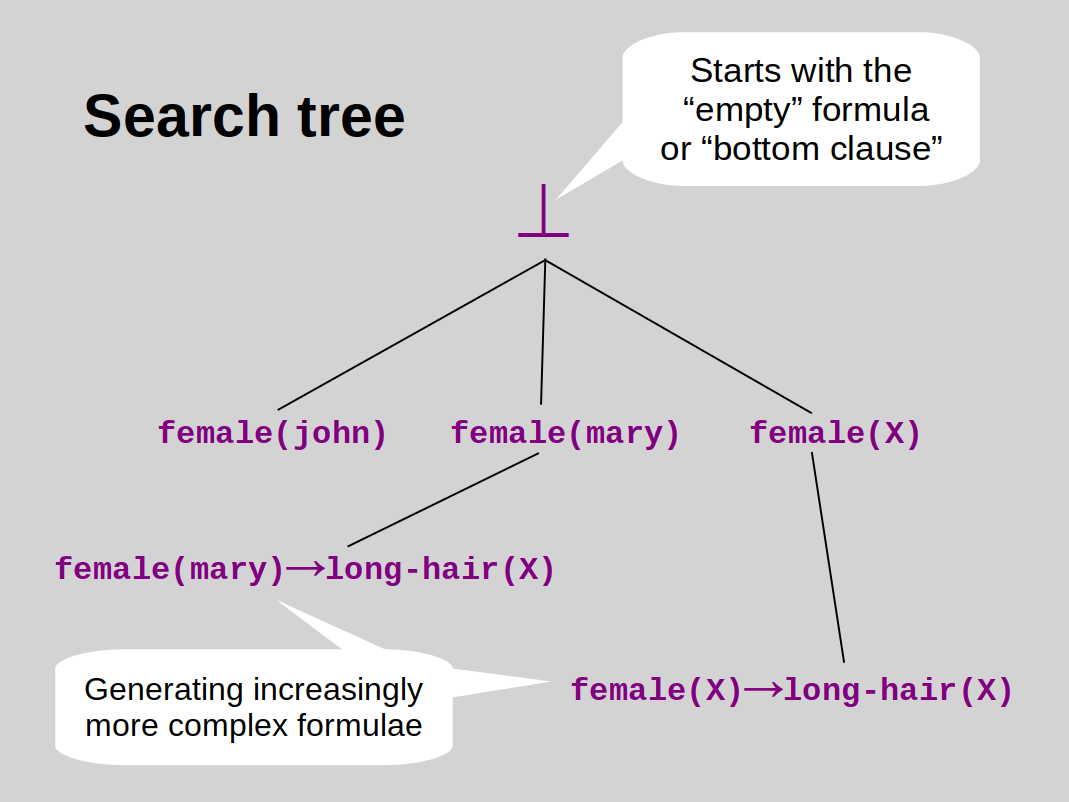
\includegraphics[scale=0.7]{induction1.png}}}
\end{equation}

A special characteristic of \textbf{mental space} is that \uline{any thought can potentially be deduced from any other thoughts}.  In other words, any two points in thoughts space may be connected by a \textbf{path} (= logic rule = action).  For example, if an agent is hungry and sees a tennis ball, the rule that ``round implies edible'' may satisfy the objective of finding food, only to be punished when one actually eats the object:
\begin{equation}
\vcenter{\hbox{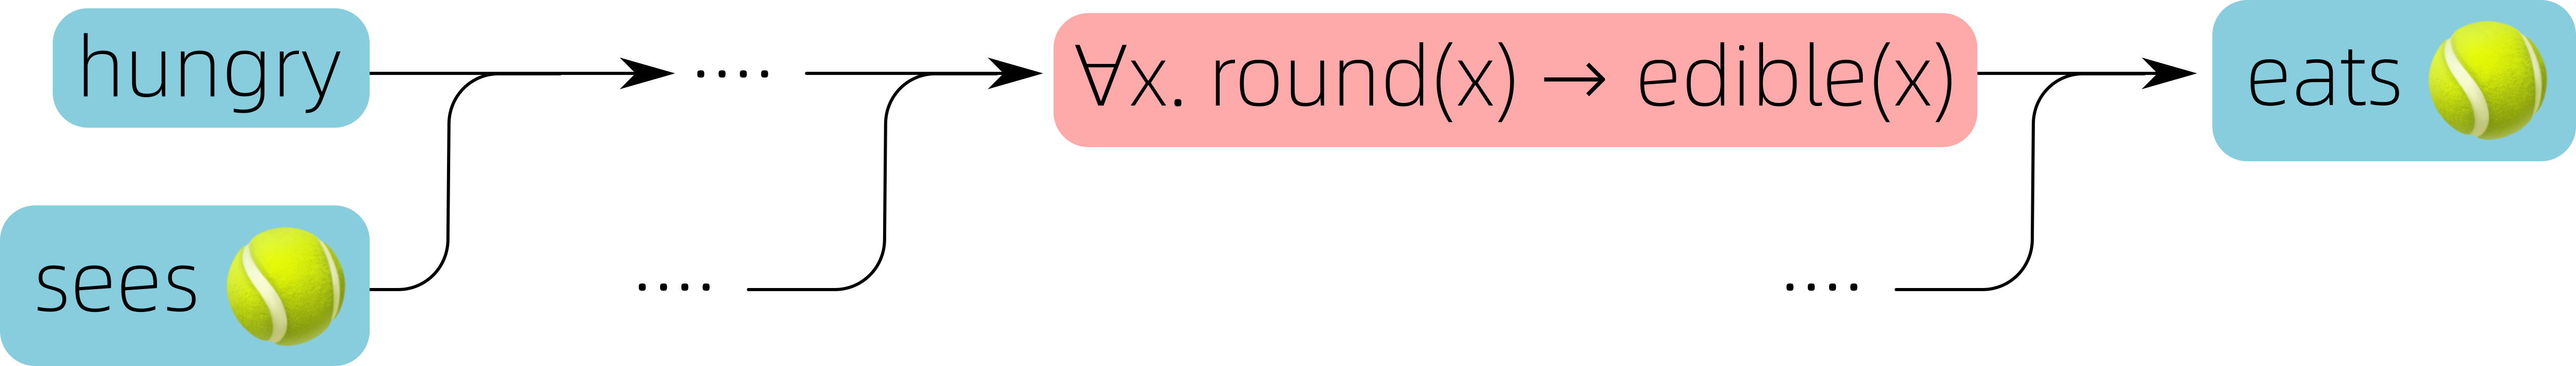
\includegraphics[scale=0.7]{tennis-ball-edible.png}}}
\end{equation}
This negative reward would back-propagate through the \textbf{inference chain}, and after many iterations, the system would eventually find the culprit rule.  In short, a logical system can get ``as crazy as it wants'' without other prior constraints.  Indeed, some geniuses arrive at non-obvious conclusions because they are a bit ``crazy''.  This property of mental space is common to all learning-reasoning systems, not just my architecture.

\end{minipage}
\end{preview}

\begin{preview}
\begin{minipage}{\textwidth}
	
\setlength{\parskip}{0.4\baselineskip}
\begin{textblock*}{20cm}(2.1cm,2cm) % {block width} (coords) 
{\color{red}{\large \textcircled{\small 3}}}
\hspace{8cm}
\color{blue}{\footnotesize \cc{强化学习的「思维空间延拓」}{Mental-Space Continuation of RL}}
\end{textblock*}

\vspace*{0.3cm} 

\subsubsection{The mind as a ``model'' of the world}

\cc{
在传统 强化学习里 有所谓 \textbf{model-based} 方法,而我们在大脑里面的 \textbf{mental model} of the world 其实是同一个概念,但由于「混合状态」的原因而被「压平」了。
}{
In traditional RL, there are \textbf{model-based} methods, and in our brain we build \textbf{mental models} of the world.  These are actually one and the same concept.
}

\cc{
	根据经典逻辑哲学,一个 (脑中的) \textbf{逻辑命题},\\
	对应于现实世界中 某个\textbf{状态}:
}{
	As is well-known in classical philosophy of logic, a logic proposition (in the mind) corresponds to certain \textbf{states} of the world:
}
\begin{equation}
\vcenter{\hbox{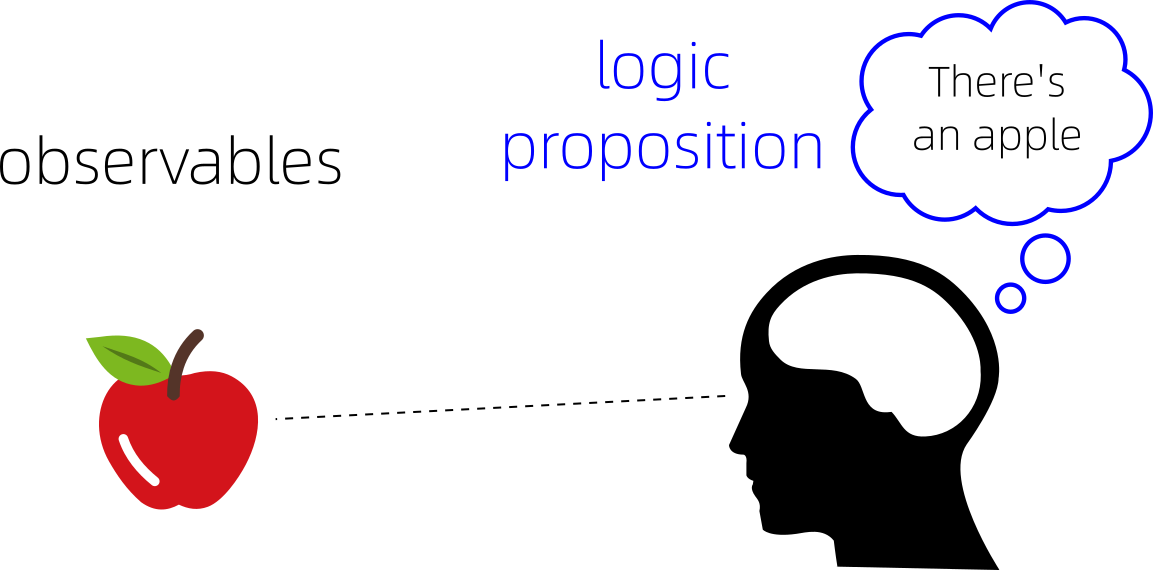
\includegraphics[scale=0.7]{logic-reality-correspondence.png}}}
\end{equation}
%\cc{
%	而这亦可以推广到,我们知道别人也有 ``other minds'' 的认知:
%}{
%	And this is still un-problematic for understanding ``other minds'':
%}
%\begin{equation}
%\vcenter{\hbox{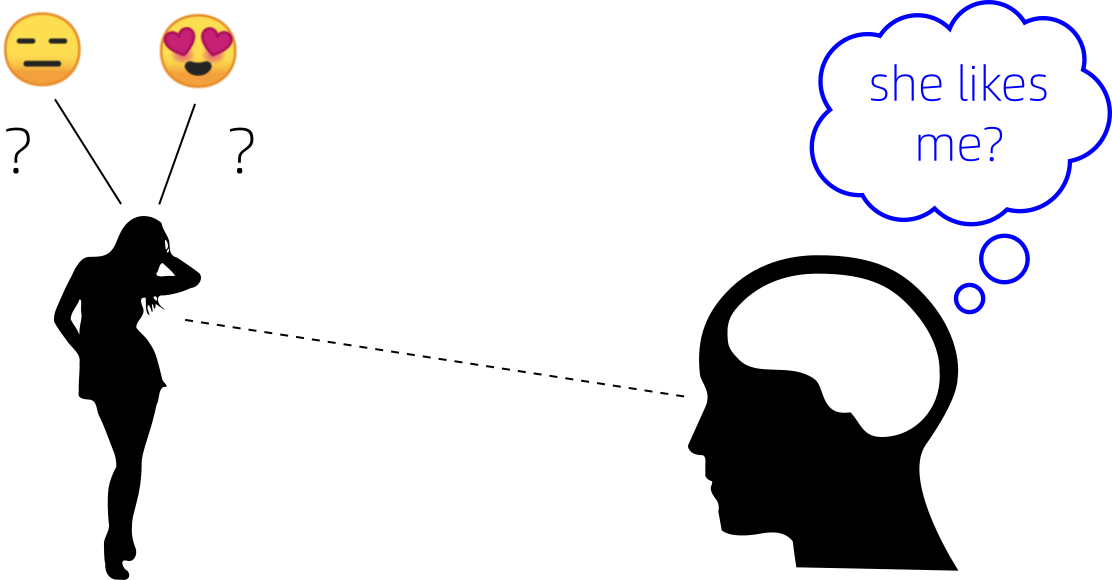
\includegraphics[scale=0.7]{other-minds.png}}}
%\end{equation}

\setcounter{mpfootnote}{2}
\cc{
	然而,在「混合状态」或 flattened view 观点下,外部世界 和 思维状态 都存在于同一个状态空间,而 思维状态 是 外部世界 的 model 或 ``theory'':\footnote{符号 $T \models M$ 的意思是: $M$ is a \textbf{model} of $T$; $T$ is a \textbf{theory} of $M$.  这是 逻辑\textbf{模型论} 的术语,有严谨的定义。}
}{
	However, in the unified or ``flat'' view, both internal and external states belong to the same state space, within which, the internal states ``model'' the external states:\footnote{The notation $T \models M$ means: $M$ is a \textbf{model} of $T$;  $T$ is a \textbf{theory} of $M$. This is rigorously defined in model theory.}
}
\begin{equation}
\vcenter{\hbox{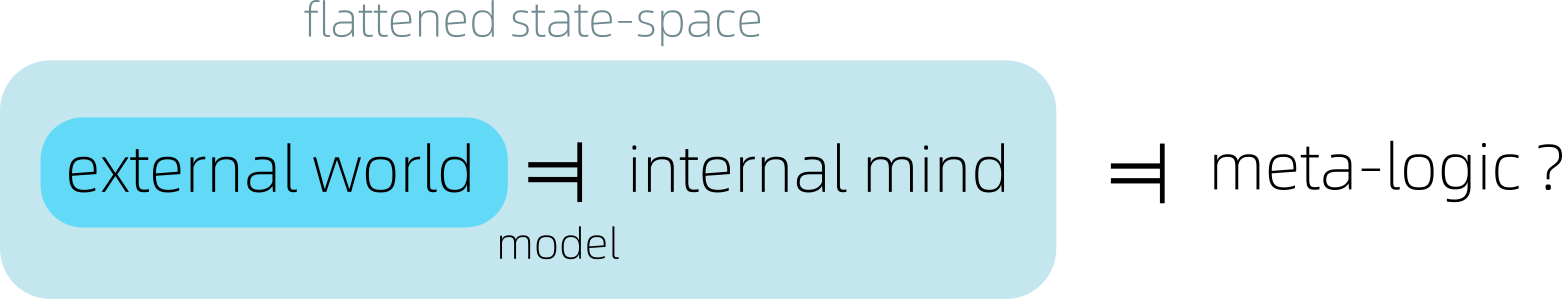
\includegraphics[scale=0.7]{model-meta-model.png}}}
\end{equation}
\cc{
	那么,混合状态空间 本身又有没有 theory 呢? 那可能是某种 \textbf{元逻辑}。
}{
	Does the unified cognitive space has its own ``theory''?  That may be some kind of \textbf{meta-logic}.  This meta-theory is a form of \textbf{inductive bias} that may be important in accelerating learning on the first-order level.
}


\footnotesize
Picture credits:\\
Human figure from www.onlinewebfonts.com licensed by CC BY 3.0\\
Thought bubble created by Catherine Please from the Noun Project
\end{minipage}
\end{preview}
\end{document}
